\documentclass[aspectratio=169,10pt]{beamer}

% --- Theme & Styling ---
\usetheme{Madrid}
\usecolortheme{whale}

\definecolor{UtmMaroon}{RGB}{128,0,32}
\definecolor{UtmGold}{RGB}{212,175,55}
\definecolor{CodeBg}{RGB}{245,245,245}
\definecolor{AccentBlue}{RGB}{24,116,205}
\definecolor{DarkGreen}{RGB}{34,139,34}

\setbeamercolor{palette primary}{bg=UtmMaroon,fg=white}
\setbeamercolor{palette secondary}{bg=UtmMaroon!85,fg=white}
\setbeamercolor{palette tertiary}{bg=UtmMaroon!70,fg=white}
\setbeamercolor{titlelike}{parent=palette primary}
\setbeamercolor{structure}{fg=UtmMaroon}

% --- Packages ---
\usepackage{colortbl}
\usepackage{tikz}
\usetikzlibrary{shapes,arrows,positioning,calc,matrix}
\usepackage{listings}
\usepackage{booktabs}
\usepackage{amsmath}

% --- Assembly Syntax Highlighting ---
\lstdefinelanguage{ARM}{
  keywords={LDR, STR, MOV, ADD, SUB, LDRB, STRB, LSL, LSR, BKPT, BX, MOVW, MOVT},
  keywordstyle=\color{UtmMaroon}\bfseries,
  comment=[l]{;},
  morecomment=[l]{@},
  commentstyle=\color{gray}\itshape,
  stringstyle=\color{DarkGreen},
  morestring=[b]",
  sensitive=false
}

\lstset{
  language=ARM,
  backgroundcolor=\color{CodeBg},
  basicstyle=\ttfamily\small,
  breaklines=true,
  frame=single,
  rulecolor=\color{black!20},
  captionpos=b
}

% --- Title Info ---
\title[Addressing Modes]{Addressing Modes: Load and Store Instructions}
\subtitle{Mastering Pre-Indexed, Post-Indexed, and Barrel-Shifter Scaling in ARM Cortex-M}
\author{Microprocessor Systems}
\date{\today}

\begin{document}

% Slide 1: Title Slide
\begin{frame}
  \titlepage
\end{frame}

% Slide 2: Broad Context - The Load-Store Model
\begin{frame}{1. Broad Context: The Load-Store Architecture}
  \begin{block}{Why Load and Store Instructions?}
    Unlike x86 CISC architectures, ARM uses a strict \textbf{Load-Store RISC Model}. ALU operations (addition, bitwise operations) \textbf{cannot directly manipulate data in RAM}. All processing occurs inside 32-bit internal registers.
  \end{block}

  \vspace{0.2cm}
  \begin{center}
    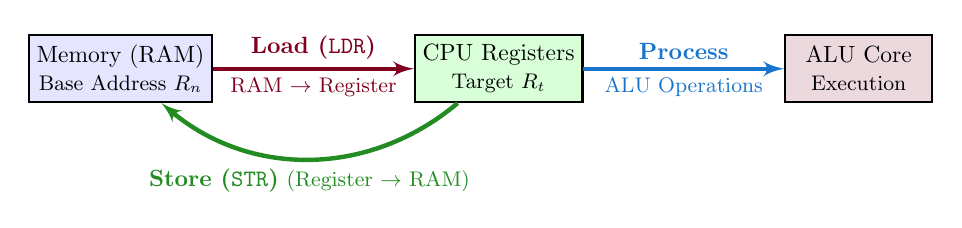
\begin{tikzpicture}[node distance=1.8cm, auto, >=latex', thick, scale=0.85, transform shape]
      \node [draw, fill=blue!10, minimum width=2.2cm, minimum height=1cm, align=center] (ram) {Memory (RAM)\\ \small Base Address $R_n$};
      \node [draw, fill=green!15, minimum width=2.2cm, minimum height=1cm, right=3cm of ram, align=center] (reg) {CPU Registers\\ \small Target $R_t$};
      \node [draw, fill=UtmMaroon!15, minimum width=2.2cm, minimum height=1cm, right=3cm of reg, align=center] (alu) {ALU Core\\ \small Execution};

      \draw[->, ultra thick, color=UtmMaroon] (ram) -- node[above] {\textbf{Load (\texttt{LDR})}} node[below] {\small RAM $\rightarrow$ Register} (reg);
      \draw[->, ultra thick, color=AccentBlue] (reg) -- node[above] {\textbf{Process}} node[below] {\small ALU Operations} (alu);
      \draw[->, ultra thick, color=DarkGreen, bend left=40] (reg) to node[below] {\textbf{Store (\texttt{STR})} \small (Register $\rightarrow$ RAM)} (ram);
    \end{tikzpicture}
  \end{center}

  \vspace{0.1cm}
  \begin{exampleblock}{Bracket Notation}
    Brackets \texttt{[ ]} act as \textbf{pointer dereferencers}: \texttt{[R1]} means \textit{"the memory location whose address is stored in R1"}.
  \end{exampleblock}
\end{frame}

% Slide 3: Visual Intuition - Pre- vs Post-Indexed
\begin{frame}{2. Visual Intuition: Pre-Indexed vs. Post-Indexed}
  \begin{columns}[T]
    \begin{column}{0.48\textwidth}
      \begin{alertblock}{Pre-Indexed: Calculate Before Access}
        Offset is added to base \textbf{before} accessing memory.
        \vspace{0.15cm}
        \begin{center}
          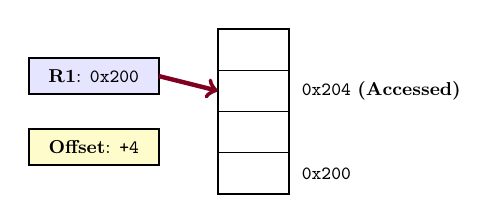
\begin{tikzpicture}[scale=0.75, transform shape]
            \draw[fill=blue!10, thick] (0,2.5) rectangle (2.2,3.1) node[midway] {\small \textbf{R1}: \texttt{0x200}};
            \draw[fill=yellow!20, thick] (0,1.3) rectangle (2.2,1.9) node[midway] {\small \textbf{Offset}: \texttt{+4}};
            \draw[thick] (3.2,0.8) rectangle (4.4,3.6);
            \draw (3.2,1.5) -- (4.4,1.5);
            \draw (3.2,2.2) -- (4.4,2.2);
            \draw (3.2,2.9) -- (4.4,2.9);
            \node[right] at (4.5, 2.55) {\small \texttt{0x204} \textbf{(Accessed)}};
            \node[right] at (4.5, 1.15) {\small \texttt{0x200}};
            \draw[->, ultra thick, UtmMaroon] (2.2,2.8) -- (3.2,2.55);
          \end{tikzpicture}
        \end{center}
        \small \textbf{Result:} Accesses calculated address \texttt{0x204}.
      \end{alertblock}
    \end{column}

    \begin{column}{0.48\textwidth}
      \begin{exampleblock}{Post-Indexed: Access First, Update After}
        Memory accessed at base address \textbf{first}, then offset added.
        \vspace{0.15cm}
        \begin{center}
          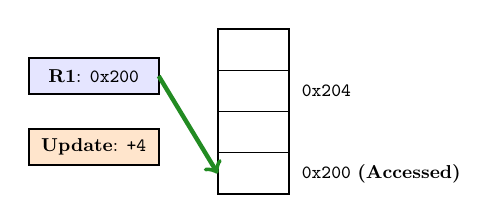
\begin{tikzpicture}[scale=0.75, transform shape]
            \draw[fill=blue!10, thick] (0,2.5) rectangle (2.2,3.1) node[midway] {\small \textbf{R1}: \texttt{0x200}};
            \draw[fill=orange!20, thick] (0,1.3) rectangle (2.2,1.9) node[midway] {\small \textbf{Update}: \texttt{+4}};
            \draw[thick] (3.2,0.8) rectangle (4.4,3.6);
            \draw (3.2,1.5) -- (4.4,1.5);
            \draw (3.2,2.2) -- (4.4,2.2);
            \draw (3.2,2.9) -- (4.4,2.9);
            \node[right] at (4.5, 2.55) {\small \texttt{0x204}};
            \node[right] at (4.5, 1.15) {\small \texttt{0x200} \textbf{(Accessed)}};
            \draw[->, ultra thick, DarkGreen] (2.2,2.8) -- (3.2,1.15);
          \end{tikzpicture}
        \end{center}
        \small \textbf{Result:} Accesses \texttt{0x200}, then updates $\text{R1} \leftarrow \texttt{0x204}$.
      \end{exampleblock}
    \end{column}
  \end{columns}
\end{frame}

% Slide 4: Offset Application & Writeback Rules
\begin{frame}{3. Offset Application \& Writeback Rules}
  \begin{center}
    \small
    \begin{tabular}{p{3.4cm} p{4.8cm} p{4.5cm}}
      \toprule
      \textbf{Addressing Mode} & \textbf{Effective Memory Address} & \textbf{Base Register Update ($R_n$)} \\
      \midrule
      \textbf{Simple Offset} & Address $= R_n + \text{offset}$ & Unchanged ($R_n$) \\
      \rowcolor{gray!15}
      \textbf{Pre-Indexed (\texttt{!})} & Address $= R_n + \text{offset}$ & Updated ($R_n \leftarrow R_n + \text{offset}$) \\
      \textbf{Post-Indexed} & Address $= R_n$ & Always Updated ($R_n \leftarrow R_n + \text{offset}$) \\
      \bottomrule
    \end{tabular}
  \end{center}

  \vspace{0.3cm}
  \begin{block}{The Writeback Indicator (\texttt{!})}
    \begin{itemize}
      \item The exclamation point \texttt{!} explicitly commands auto-update (writeback) for pre-indexed access.
      \item Post-indexed access \textbf{implicitly updates} the base register without requiring a \texttt{!} symbol.
    \end{itemize}
  \end{block}
\end{frame}

% Slide 5: Detailed Syntax - Immediate Offsets
\begin{frame}[fragile]{4. Detailed Syntax: Immediate Offsets (\#imm)}
  \begin{columns}[T]
    \begin{column}{0.48\textwidth}
      \textbf{1. Simple Immediate Offset}
      \begin{lstlisting}
LDR R0, [R1, #4]
@ Effective Address = R1 + 4
@ R1 remains unchanged
      \end{lstlisting}

      \vspace{0.2cm}
      \textbf{2. Pre-Indexed with Writeback}
      \begin{lstlisting}
LDR R0, [R1, #4]!
@ Effective Address = R1 + 4
@ R1 auto-updates: R1 = R1 + 4
      \end{lstlisting}
    \end{column}

    \begin{column}{0.48\textwidth}
      \textbf{3. Post-Indexed (Implicit Writeback)}
      \begin{lstlisting}
LDR R0, [R1], #4
@ Access Address = R1
@ After load: R1 = R1 + 4
      \end{lstlisting}

      \vspace{0.2cm}
      \begin{alertblock}{Syntax Rule of Thumb}
        \begin{itemize}
          \item Offset \textbf{inside} brackets $\rightarrow$ Pre-indexed
          \item Offset \textbf{outside} brackets $\rightarrow$ Post-indexed
          \item Trailing \texttt{!} $\rightarrow$ Pre-indexed writeback
        \end{itemize}
      \end{alertblock}
    \end{column}
  \end{columns}
\end{frame}

% Slide 6: Register Offsets
\begin{frame}[fragile]{5. Dynamic Indexing: Register Offsets ($R_m$)}
  \begin{block}{Why Register Offsets?}
    When array indices or offsets are computed dynamically at runtime, a secondary register $R_m$ replaces the constant immediate \texttt{\#imm}.
  \end{block}

  \vspace{0.2cm}
  \begin{columns}[T]
    \begin{column}{0.48\textwidth}
      \textbf{Simple Register Offset}
      \begin{lstlisting}
LDR R0, [R1, R2]
@ Address = R1 + R2
@ R1 remains unchanged
      \end{lstlisting}

      \vspace{0.2cm}
      \textbf{Pre-Indexed Register Offset}
      \begin{lstlisting}
LDR R0, [R1, R2]!
@ Address = R1 + R2
@ R1 = R1 + R2
      \end{lstlisting}
    \end{column}

    \begin{column}{0.48\textwidth}
      \textbf{Post-Indexed Register Offset}
      \begin{lstlisting}
LDR R0, [R1], R2
@ Access Address = R1
@ R1 = R1 + R2
      \end{lstlisting}

      \vspace{0.2cm}
      \begin{exampleblock}{Use Case}
        Ideal for stepping through arrays where element stride is stored in a register ($R_2$).
      \end{exampleblock}
    \end{column}
  \end{columns}
\end{frame}

% Slide 7: Dedicated LSL Slide - Scaled Register Offsets & Barrel Shifter
\begin{frame}[fragile]{6. Scaled Register Offsets \& The Barrel Shifter}
  \begin{block}{Hardware Barrel Shifter Integration}
    ARM cores integrate a hardware \textbf{Barrel Shifter} directly into the memory address generation unit. This allows multiplying an index register by $2^n$ in the \textbf{same single clock cycle} as memory access.
  \end{block}

  \vspace{0.2cm}
  \begin{columns}[T]
    \begin{column}{0.52\textwidth}
      \textbf{Assembly Syntax with Bitwise Shift}
      \begin{lstlisting}
@ Address = R1 + (R2 * 4)
LDR R0, [R1, R2, LSL #2]

@ Pre-indexed with writeback
STR R0, [R1, R2, LSL #2]!

@ Post-indexed scaling
LDR R0, [R1], R2, LSL #2
      \end{lstlisting}
    \end{column}

    \begin{column}{0.44\textwidth}
      \begin{exampleblock}{C Data Type Scale Mapping}
        \begin{itemize}
          \item \texttt{LSL \#1} ($\times 2$): 16-bit \texttt{short}
          \item \texttt{LSL \#2} ($\times 4$): 32-bit \texttt{int} / pointers
          \item \texttt{LSL \#3} ($\times 8$): 64-bit \texttt{double}
        \end{itemize}
      \end{exampleblock}

      \vspace{0.1cm}
      \small \textbf{Efficiency:} Eliminates explicit \texttt{MUL} instructions before array access!
    \end{column}
  \end{columns}
\end{frame}

% Slide 8: Constant Loading & Literal Pools
\begin{frame}[fragile]{7. Constant Loading \& PC-Relative Literal Pools}
  \begin{alertblock}{Architectural Limitation}
    In 32-bit ARM instructions, immediate values are limited to 12 bits (8-bit value rotated). Arbitrary 32-bit memory addresses (e.g., \texttt{0x20000000}) \textbf{cannot fit inside a standard MOV instruction}.
  \end{alertblock}

  \vspace{0.2cm}
  \begin{columns}[T]
    \begin{column}{0.48\textwidth}
      \textbf{Method 1: Assembler Pseudo-Instruction}
      \begin{lstlisting}
LDR R0, =0x20000000
LDR R1, =MY_DATA_LABEL
      \end{lstlisting}
      \small Assembler converts this into a \textbf{PC-relative load} from a near-by \textit{Literal Pool}:
      \begin{lstlisting}
LDR R0, [PC, #offset]
      \end{lstlisting}
    \end{column}

    \begin{column}{0.48\textwidth}
      \textbf{Method 2: Two-Instruction Construct}
      \begin{lstlisting}
@ Load lower 16 bits
MOVW R0, #0x0000
@ Load upper 16 bits
MOVT R0, #0x2000
      \end{lstlisting}
      \small Uses ARMv7-M \texttt{MOVW}/\texttt{MOVT} instructions to build a 32-bit constant directly into $R_0$.
    \end{column}
  \end{columns}
\end{frame}

% Slide 9: Syntax Decision Tree & Cheatsheet
\begin{frame}{8. Syntax Decision Tree \& Summary}
  \begin{center}
    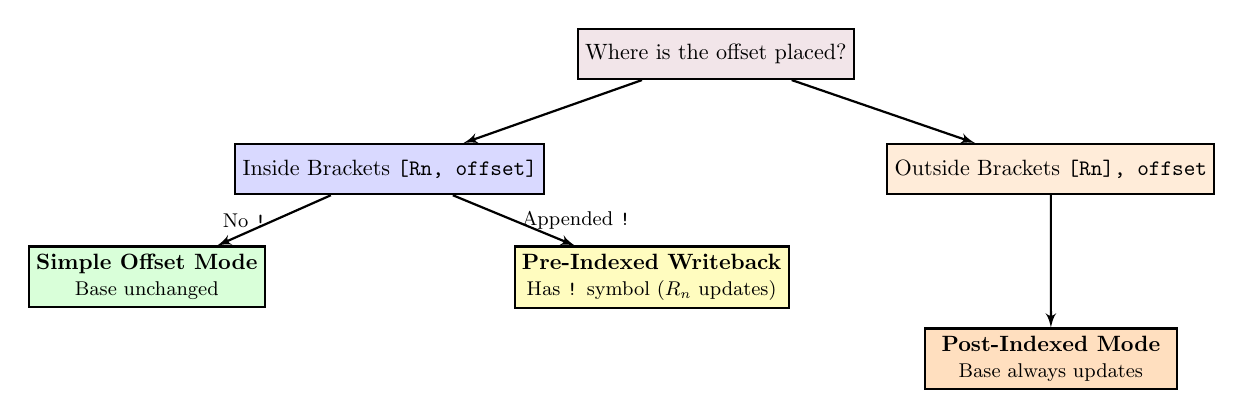
\begin{tikzpicture}[node distance=1.5cm, auto, >=latex', thick, scale=0.8, transform shape]
      \node [draw, fill=UtmMaroon!10, minimum width=3.5cm, minimum height=0.8cm, align=center] (q1) {Where is the offset placed?};

      \node [draw, fill=blue!15, minimum width=3.8cm, minimum height=0.8cm, below left=1cm and 0.5cm of q1, align=center] (in) {Inside Brackets \texttt{[Rn, offset]}};
      \node [draw, fill=orange!15, minimum width=3.8cm, minimum height=0.8cm, below right=1cm and 0.5cm of q1, align=center] (out) {Outside Brackets \texttt{[Rn], offset}};

      \node [draw, fill=green!15, minimum width=3.5cm, minimum height=0.8cm, below left=0.8cm and -0.5cm of in, align=center] (sim) {\textbf{Simple Offset Mode}\\ \small Base unchanged};
      \node [draw, fill=yellow!25, minimum width=3.5cm, minimum height=0.8cm, below right=0.8cm and -0.5cm of in, align=center] (pre) {\textbf{Pre-Indexed Writeback}\\ \small Has \texttt{!} symbol ($R_n$ updates)};

      \node [draw, fill=orange!25, minimum width=4cm, minimum height=0.8cm, below=2.1cm of out, align=center] (post) {\textbf{Post-Indexed Mode}\\ \small Base always updates};

      \draw[->] (q1) -- (in);
      \draw[->] (q1) -- (out);
      \draw[->] (in) -- node[left] {\small No \texttt{!}} (sim);
      \draw[->] (in) -- node[right] {\small Appended \texttt{!}} (pre);
      \draw[->] (out) -- (post);
    \end{tikzpicture}
  \end{center}

  \vspace{0.2cm}
  \begin{exampleblock}{Quick Memory Rule}
    \textbf{Pre-Indexed:} Calculate address first $\rightarrow$ access memory. \\
    \textbf{Post-Indexed:} Access memory first $\rightarrow$ update pointer.
  \end{exampleblock}
\end{frame}

\end{document}
